%\documentclass[titlepage,a4paper,12pt]{book}
%\usepackage[utf8]{inputenc}
%\usepackage[catalan]{babel}
%\usepackage{graphicx}
%\usepackage{marvosym}
%\usepackage{listings}
%\usepackage{textcomp}
%\usepackage[]{url}
%\usepackage[]{color}
%\begin{document}
%\tableofcontents

\section{Introducció} % (fold) Objectius?
	\label{sec:Introduccio}
	Un altre problema on hem aplicat Algoritmes evolutius és en el descobriment
	de fàrmacs \texttt{de novo}.  \texttt{De novo} és el nom que es dóna a les
	tècniques relacionades amb el descobriment des de zero , és a dir, on no es té
	prèviament cap lligand a imitar.

	La situació és la següent.  En determinades situacions, es disposa d'un
	esquelet o \textit{scaffold} d'una molècula que se sap que té certa
	activitat, però no es disposa amb seguretat de algunes
	\textit{ramificacions} (R), que són les parts de la molècula que, sense
	canviar la seva estructura general, ni la seva activitat (si el ``core''
	s'assembla, probablement tindrpàn una activitat similar), faran que es pugui
	``enganxar'' millor en el target.  Les ramificacions que poden anar en cada
	posició són conegudes (en la majoria de casos).

	En certa manera, podríem dir que és com ``decorar'' l'esquelet de la
	molècula per a fer-lo més apte per a la unió amb la seva diana (o target).

	Un dels problemes que tenen els mètodes actuals són els grans costos
	que es deriven d'aquest procés, ja que el que es fa és sintetitzar TOTES les
	possibles variants i combinacions de substituients, i mesurant
	experimentalment l'activitat de cadascun d'ells, buscant la que dona major
	activitat.
	%la energia XXX (disipada?) s'intenta buscar la que minimitza aquesta.

	si tenim un esquelet com el següent, amb 3 punts on unir substituients,
	i 4 posibles ``blocs de construcció'' (building blocs) per a cada R, la
	combinatiòria ens dóna que necessitarem sintetitzar aproximadament $4^3 =
	64 $, però si el número creix una mica, el creixement és exponencial, fent
	molt costós el procediment.

	Si pensem que la qualitat del resultat final depèn de les
	ramificacions escollides per a cada $R1..RN$, podem anar una mica més enllà i
	intentar fer una aplicació que ens ajudi i ens guii a trobar un lligand amb
	bona activitat explorant només una petita part de l'espai de cerca.
	
	\texttt{La idea en aquest programa és doncs, construir un algoritme genètic
	interactiu que ens permeti arribar a la millor tria de ramificacions (o
	alguna de molt bona) sintetitzant només una petita part del espai de búsqueda.}

	Per a avaluar la qualitat de una combinació, no hi ha més remei que
	sintetitzar la molècula en qüestió en el laboratori i retornar el resultat
	al programa.  Així doncs, es tracta d'un algorisme genètic interactiu que
	ens guiarà les proves que hem de fer a través dels creuaments i les
	mutacions, trobant ``relacions'' (epistàcia) entre els diferents
	ramificacions, i aconseguint resultats bons explorant només una petita part
	del espai de búsqueda.

	Una altre objectiu d'aquest programa, ha estat convertir-lo en un
	``framework'' d'algorismes genètics.  Veient que la funció de fitness és una
	funció que executa l'usuari, i ell és qui puntúa cadascuna de les
	combinacions, s'ha intentat anar més enllà i aconseguir una aplicació que
	pugui ser utilitzada no només en aquest context, sinó en qualsevol que ens
	podem trobar en un futur, sempre i quan requereixi uns operadors similars.

	Una altra manera d'imaginar-se aquest enfoc \emph{meta} és pensar-ho com si
	separéssim la funció fitness de la resta del procés d'algoritme genètic.
	L'únic que necesita el algoritme genètic és un receptor de dades (en el
	nostre cas inicial és l'usuari), que donada una entrada, doni una
	sortida (fitness).  Si es mira d'aquesta manera, no estem fent més que
	desacoblar l'avaluació del procés de creuaments, mutacions i reproducció.

	Fins a aquest punt, podríem utilitzar algun sistema amb ``callbacks'', on
	l'usuari simplement entri els fitness als diferents individuus (combinacions
	de ramificacions), però com que l'avaluació no és instantànea, el programa no
	només ha de ser interactiu en el sentit clàssic del terme (inici-interacció-fi),
	sinó que ha de permetre aturar-se i més endevant, tornar a rependre el curs
	del algoritme evolutiu. 

	Una vegada estem en aquest punt, la següent evolució lògica és la
	deslocalització també espaial de les 2 parts.  Donat que el procés
	d'avaluació d'una combinació de substituients donada pot trigar dies, el coll
	d'ampolla és clarament aquest, permetent-nos així separar algorisme
	genètic i fitness a través d'una xarxa, i permetent convertir el sistema en
	un servei web, accessible des d'arreu del món.

	Tot i que la gestió d'això només ens implica implementar el sistema com a
	servei web (SOAP) i tenir una bona gestió d'usuaris i projectes, es veu
	clarament que el que comença essent una aplicació per a solucionar un
	problema concret, s'ha anat abstraient i generalitzant fins al punt de
	convertir-se en un programa molt més potent, ja que ara abarca un espectre
	molt més gran de problemes pels quals està capacitat resoldre.

	Tot seguit s'explica més a fons algun concepte bàsic de la química
	combinatòria, seguit dels detalls d'implementació de la aplicació.

% section Introducció (end)

\section{Context Químic} % (fold)
	\label{sec:Context Quimic}

	\subsection{Química combinatòria}
	Típicament es pot dividir el desenvolupament d'un fàrmac en tres grans
	fases. Una primera \emph{in vitro}, en la qual es treballa exclusivament en
	laboratoris de síntesi i disseny de biomolècules. Una altra posterior
	\emph{in vivo}, en la que es treballa amb models biològics o en animals.
	Finalment, l'última fase que ja és en humans. Cada cop que es passa de fase,
	la precisió dels models és més acurada i més fidel al pacient final.
	Malauradament el cost també pateix un gran augment cada cop que s'avança en
	aquesta escala. Amb la qual cosa això ha propiciat el naixement de
	filosofies de disseny \emph{in vitro} tals com la química combinatòria.

	La química combinatòria és una tècnica molt emprada en el disseny de nous
	fàrmacs. La filosofia original consta de dues parts, primer una on es proven
	milers i fins i tot milions de compostos per veure si algun d'ells
	aconsegueix mínimament l'objectiu que s'està buscant. Un cop trobat un
	\emph{hit}, s'entra en una segona fase d'optimitzacions d'aquest compost.

	Aquesta filosofia s'ha ajudat molt de la biotecnologia moderna. S'han
	automatitzat tots els processos que abans es feien manualment, de manera que
	el rendiment (\emph{throughput}) s'ha multiplicat en variïs ordres de
	magnitud. Però això no ha evitat que els costos de desenvolupament d'un nou
	fàrmac també hagen augmentat en varis ordres de magnitud.

	\subsection{Química combinatòria virtual}

	L'augment de costos i de temps de les fases \emph{in vitro}, ha donat lloc
	al naixement a una fase prèvia, coneguda com \emph{in silico}. En aquesta
	nova fase, els models emprats fins i tot són de menor qualitat que els models
	emprats en la fase \emph{in vitro}.  L'avantatge d'aquesta fase rau en que
	els costos i temps es redueixen, ja que un supercomputador pot provar de
	forma molt ràpida un gran nombre de compostos.

	Aquest fet ha donat lloc a la química combinatòria virtual, on ara els
	milions de compostos són provats per via computacional, i sols uns quants
	centenars o desenes de \emph{leaders} passaran a la fase \emph{in vitro}.

	Aquestes tècniques han començat a establir-se en el disseny de fàrmacs des
	de fa uns 10 anys. Recentment està sorgint altra tendència més innovadora i
	prometedora que és introduir elements d'intel·ligència artificial en aquesta
	fase. La vessant de la intel·ligència artificial que està sent més
	utilitzada en aquests tipus de problema són els algorismes de cerca, i
	concretament, algorismes evolutius. Encara que, no es descarten altres àrees
	de la intel·ligència artificial com l'aprenentatge artificial, etc.  Per
	exemple, per desenvolupar models biològics virtuals, aprendre les
	estructures que actuen com a bons fàrmacs, o resolucions d'estructures
	tridimensionals. 

\subsubsection{El nostre problema} % (fold)

	En el nostre cas, posicionem el nostre programa en la fase d'optimització,
	una vegada es disposa d'un esquelet que presenta certa activitat i tenint
	uns punts d'on poden penjar seqüències d'atoms, anomenades ramificacions (o
	substituients), anar provant d'enganxar els diferents substituients en
	cadascun dels punts definits com a inicis dels substituients.

	En el proccés de descobriment de fàrmacs, no només és
	necessari trobar un compost que reaccioni favorablement a una molècula
	objectiu, sinó que també ha de reunir certes propietats per tal que
	un principi actiu es pugui convertir en un fàrmac aplicable.  	

	Aquestes propietats , moltes vegades vénen determinades per aquestes
	branques o ramificacions, que fan que un mateix esquelet, sigui més o menys
	absorbible pel cos, o pot donar-li propietats negatives per als nostres
	objectius.

	Quan en un laboratori, se sap sintetitzar un esquelet (scaffold), la
	producció de les diferents variants d'aquest esquelet és molt senzilla.  És
	per això que té sentit explorar les possibles combinacions de Rs una vegada
	s'ha fet la inversió de desenvolupar el procediment per a sintetitzar aquest
	esquelet.

	El que hem fet aquí és crear un programa que mitjançant un algorisme
	genètic ens ajuda a trobar un conjunt de ramificacions que optimitzen el
	fàrmac.

	El problema que hem analitzat en un principi és el de XXX
	on tenim un espai de búsqueda de 15360 possibles combinacions.

	Com es veurà a durant el capítol, hem volgut anar més enllà i no limitar-nos
	només a solucionar aquest problema, però per aquest treball, els resultats
	presentats sí que seràn respecte a aquest cas.
% section Context Químic (end)

\section{Procediment informàtic} % (fold)
\label{sec:Procediment informatic}

En aquesta aplicació, no ha estat tant complex d'implementar l'algorisme genètic
com tot l'entorn (framework) que permet fer del \texttt{nucli} una part molt
flexible i accessible des de tot arreu (web, consola).

El diseny de \texttt{Chiron}, ha hagut de estar molt pensat, i de fet, s'ha vist
modificat a mesura que avançava la seva implementació per problemes que s'han
trobat en tecnologies que pensàvem que serien suficientment flexibles per a les
nostres necessitats, i després s'ha vist que no eren del tot adecuades per a
complir els requeriments.

Començarem amb el workflow que facilita l'us de Chiron i n'extraurem els
diferents casos d'ús, i després s'anirà describint el procés que s'ha realitzat
per a implementar-ho.

\subsection{Funcionament} % (fold)
\label{sub:Funcionament}

Un usuari, en començar un projecte, ha de poder crear un experiment nou.  Aquest
experiment ha d'estar lligat, òbviament a aquest usuari, amb el que ens obliga
també a poder fer altes, baixes i modificacions dels usuaris que tenen accés a
la aplicació.

Les altes, baixes i modificacions de usuaris no les gestiona el propi
\texttt{Chiron}, ja que la aplicació que dona accés a Chiron és qui s'encarrega
de controlar els accessos a aquests.  Chiron únicament utilitza la base dades
aquesta, per saber quin usuari és el que està utilitzant el programa, i fa totes
les accions en el seu nom.

La creació de experiments nous sí que és una labor de Chiron, i és a partir
d'aquest moment on Chiron s'encarrega de registrar els events.

Per a la creació d'un nou experiment, Chiron necessita únicament el número de
ramificacions que conté l'esquelet (R1 \dots RN), el número d'al·lels diferents que
poden estar en cadascuna de les ramificacions, la mida de la població, i un booleà
indicant si volem que Chiron recordi (cachegi) els resultats o no.  Amb aquestes
dades, Chiron en té prou per començar l'experiment.  És clar que també demanarà
un nom per al que l'usuari s'hi pugui referir.

En aquest punt, hi ha dues coses que poden sorprendre, i seguidament s'expliquen
els perquès:

\begin{itemize}
	\item \textbf{No necessitem l'scaffold}. Per a Chiron, l'esquelet (scaffold)
	que usem no té la més mínima importància, ja que sempre serà una part fixa,
	i no ens aportarà res per a la nostra aproximació al problema.  És per això
	que el programa, tot i guardar-se'l per a futura referència, no l'usa en tot
	el procés per a fer càlculs.

	\item \textbf{Perquè decidir si guardem els resultats previs?}
	Aparentment, sempre que calculem un individuu nou, hauríem de guardar-nos
	els resultats obtinguts per si més endevant surt el mateix element.  El fet
	que ens fa donar-li la opció al usuari és que l'avaluació de la activitat
	d'una molècula, es fa en un laboratori, i segons el tipus d'experiments que
	es fan, els resultats només tenen valor uns en relació amb els altres.  Si
	és així, al usuari no li interessa que es guardin els valors ja calculats,
	ja que si en properes generacions del algorisme genètic torna a apareixer la
	mateixa combinació de substituients, s'haurà de calcular de nou.
\end{itemize}

Una vegada l'usuari ha creat el nou experiment, se li proposen unes quantes
molècules a avaluar (tantes com hagi decidit l'usuari com a mida de la
població).

Al cap d'un temps, quan l'usuari ha avaluat les molècules proposades per Chiron,
aquest retornarà a la interfície de Chiron, identificarà l'experiment, i posarà
valors a cadascuna de les molècules avaluades.  Una vegada les tingui TOTES
avaluades (sinó estan totes, Chiron no deixarà passar d'aquest punt), s'activarà
la opció de \texttt{fer una altra iteració}.  

En aquest punt, a partir de les dades que tenim, Chiron fa una iteració i
presentarà al usuari una nova generació de molècules, fent creuaments i
mutacions sobre les molècules que tinguem avaluades.

Com que el workflow d'aquest programa no és ``continu'' en el sentit que el
programa es manté viu durant tot el procés, les dades que volem guardar (encara
que siguin només temporals o internes per a un experiment determinat), s'han
d'emmagatzemar en una base de dades, ja que les tècniques de memoizing %apartat pholus
perden la informació d'execució en execució, i no funcionarien en aquest cas.

Per a aquesta tasca s'ha utilitzat un servidor remot MySql.
%estructura de taules

La inicialització de la primera generació és aleatoria. En el cas que en la
primera generació no hi hagi cap molècula que presenti la més mínima activitat
(no superen un llindar donat), Chiron no segueix el curs normal de mutacions i
creuaments, ja que això ens dóna lloc a un intent de convergència que no ens
interessa.  Per exemple, si tenim una població de 30 individuus i tots tenen
fitness 0, Chiron intentarà fer creuaments entre ells aleatoris (ja que cap
d'ells guanya sobre els altres).  No només això sinó que al fer això, molts dels
individuus de la següent generació seran iguals als ja evaluats, ja que hem
reduit molt l'espai de búsqueda sobre el que explorem.

Si avaluéssim funcions matemàtiques contínues i amb un gradient clar fins al
millor resultat (o els millors resultats), com en la Figura \ref{fig:normal}, no
tindríem aquest problema, però els nostres casos són, en la gran majoría, casos
hiperdimensionals, on tenim un espai de búsqueda molt gran però els pous amb
activitat són molt pocs (i estrets), i hem d'intentar arribar a aquests pous
primer, i després optimitzar per les vies del algoritme genètic (Figura
\ref{fig:dificil}).

\begin{figure}[h]
	\begin{center}
		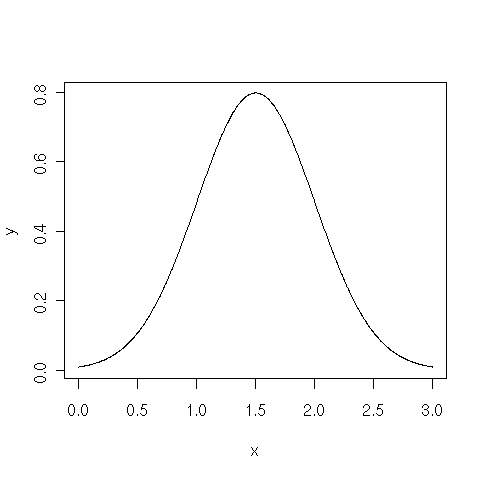
\includegraphics[scale=0.5]{chiron/normal.png}
	\end{center}
	\caption{normal}
	\label{fig:normal}
\end{figure}

\begin{figure}[h]
	\begin{center}
		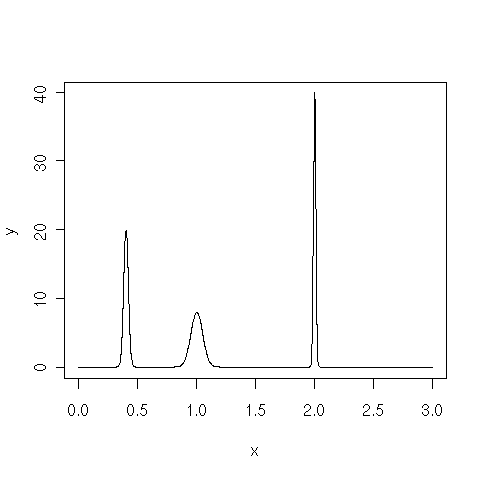
\includegraphics[scale=0.5]{chiron/pics.png}
	\end{center}
	\caption{Suma de Gaussianes difícil de trobar per Chiron} 
	\label{fig:dificil}
\end{figure} 

La solució que s'ha adoptat ha estat la de generar una població d'individuus
nova, sense tenir en compte ĺa generació anterior, com si es comencés un
experiment nou.  Fent això evitem que l'algoritme genètic estigui ``viciat'' de
bon principi, i maximitzem les probabilitats de trobar algun pou d'energia.
%XXX : Convergencia prematura

Les proves de correctesa del programa, s'han fet amb funcions matemàtiques
contínues, per tal de saber del cert que l'algorisme funciona bé i més endevant
s'ha provat amb el cas real de química combinatiòria.

%Els resultats obtinguts d'aquestes funcions també seràn exposats més endevant
%en l'apartat de resultats. 

\subsubsection{Testeig} % (fold)
\label{ssub:Testeig}

Hi ha un conjunt de funcions matemàtiques que es consideren ``típiques'' per a
usarles com a ``problemes joguina'' (toy problems), per exemple, s'ha provat
l'algoritme evolutiu representant una funció on cada al·lel només té dos
possibles valors , 0 i 1, i la funció únicament suma els bits dels cromosomes.
El que es busca en aquesta funció, és maximitzar o bé minimitzar el resultat de
la suma de bits.  Aquest, tot i ser un exemple trivial, ens serveix per
saber si l'algorisme evolutiu funciona correctament.  Aquest exemple també ens
serveix perquè les mutacions i creuaments utilitzats són els mateixos que
utilitzem en la versió final de la aplicació.

Els resultats obtinguts són bons, arribant al millor resultat (tot uns) o a un
dels millors explorant només un percentatge de aproximadament el  10\% de
l'espai de búsqueda.

La funció de la suma de bits és una funció trivial per a cualsevol algorisme
evolutiu, donada la seva simplicitat.  És per això que després de provar amb
aquesta funció, hem provat funcions més complicades d'optimitzar, fins a arribar a
les conegudes com a ``funcions trampa''(\ref{EU2009}).  Les funcions trampa són funcions que
tenen característiques que fan molt difícil als AE trobar el màxim/mínim global,
tenint el millor resultat global envoltat de resultats molt dolents, i tenint un
màxim/mínim local ``fàcil'' d'arribar-hi en un extrem, apartant les solucions de
l'òptim global.  Una de les funcions trampa que hem provat, és la de mapejar en
un vector de bits una valoració determinada per a cada suma de bits.  Per
exemple, donat un vector de 5 posicions:

 % theme=Berlin;caption_top=1;caption=Exemple tanimotos
 % bits a 1 & valor
 % 0 & 1
 % 1 & 2
 % 2 & 3
 % 3 & 4
 % 4 & 5
 % 5 & 0

\begin{table}
\centering
\caption{Funció trampa}
\begin{tabular}{|r|r|}
\hline
\multicolumn{1}{|c|}{\textbf{bits a 1 }} & \multicolumn{1}{c|}{\textbf{ valor}} \\
\hline
\hline
0 & 1 \\
1 & 2 \\
2 & 3 \\
3 & 4 \\
4 & 5 \\
5 & 0 \\
\hline
\end{tabular}
\end{table}


L'ideal en aquest cas és trobar el vector que té 5 bits a 1, és a dir, busquem
minimitzar la funció.  Això, clarament és una trampa per a l'algorisme genètic,
ja que al fer els creuaments entre dos cromosomes que tenen una bona puntuació,
fa que els resultants, siguin molt dolents. És una manera d'enganyar al
algoritme evolutiu que ens serveix per a saber si aquest és prou robust per a
trobar un resultat bo.  En aquests casos, l'elitisme, és molt determinant per a
obtenir bons resultats.
% subsubsection Testeig (end)

%SOAP
\subsubsection{Funció fitness configurable} % (fold)
\label{ssub:Funcio fitness configurable}

Un altre aspecte important de Chiron és la versatilitat que té per a executar-se
amb diferents funcions de fitness.  Com s'ha explicat en la introducció del
capítol, Chiron permet avaluar manualment cadascun dels elements.  Donat que una
avaluació d'una molècula pot portar dies o setmanes, l'algorisme genètic ha de ser
capaç de mantenir l'estat i congelarse a cada iteració.

Les llibreries usades (eodev), estan preparades per a mantenir l'estat en arxius
de text pla, però ho fan en el moment que s'ha acabat de executar la funció
avaluació de tots els individus d'una generació.  Per a poder aturar la
execució abans (a nivell lògic), el que hem disenyat és un sistema per a
recollir i posar dades automàticament en els arxius de estat.  eodev està
programat en c++, i per tant, la funció de fitness ha de ser sempre la mateixa
ja que només volem tenir una instància de \texttt{Chiron} per executar, i no pas
una per a cada projecte que es faci.  El que hem fet per a solucionar aquesta
qüestió és ``anul·lar'' la funció de fitness fent que sigui una stub, que dona
fitness zero a tots els individus que avalua.  Configurant Chiron per a què
faci una sola generació, aconseguim guardar l'estat en un arxiu, amb els
paràmetres del algorisme genètic, les llavors (seed), i els individus de la
generació actual.  Llavors, el programa que executa el nucli de Chiron pot
parsejar l'arxiu, i insertar els elements en una base de dades (ens interessa
tenir un històric de tots els elements avaluats en generacions prèvies).
Aquests resultats són els que es presenten al usuari, que pot recuperar cuan
vulgui ja que la recuperació de les dades es fa desde la base de dades MySql.

Quan l'usuari disposa de dades sobre les molècules, les pot introduir a través
d'una interfície, i tornar a executar una generació.

Si l'usuari ha configurat el projecte perquè mantingui els valors d'avaluacions
passades, en el moment que Chiron detecta una molècula que ja ha estat avaluada,
no li presenta al usuari, i és Chiron qui s'encarrgarà de afegir el resultat en
el moment de la següent generació.

%subsub?  PRoblemes d'inicialització.

En  molts casos reals, ens trobem que tenim una immensa majoria de valors iguals
com a resultat de les avaluacions.  Aquests resultats són per les molècules que
o bé no poden ser sintetitzades, o bé no superen un llindar mínim d'activitat.

Això ens ha suposat un gran problema perquè si avaluem la primera generació i
tots els elements tenen el mateix fitness (0), la següent població que Chiron
suggerirà serà una població tal que haurà sortit de creuar i mutar la primera
població aleatoriament entre ella.  Aquest procediment ens provoca una
convergència prematura que no desitgem, ja que el que passa en realitat és que
encara no hem mostrejat cap molècula que ens doni un mínim d'activitat amb el
que poder ``jugar''.

Problemes d'aquestes característiques només es donen en casos on l'espai de
búsqueda és molt gran comparat amb el número de elements que tenen resultats
diferents de 0.

Per exemple, si volguéssim trobar, en el problema de la suma de bits una
configuració concreta (10101), o bé trobar elements amb unes certes
característiques (que sumin 3), i tots els elements que ho compleixen tenen
fitness 1 i els que no, tenen fitness 0, ens trobariem amb problemes similars.

Aquest problema, l'hem solucionat provocant que Chiron resetegi l'experiment
(recordant les molècules avaluades en la base de dades), i torni a donar una
població d'individuus aleatòria.  Així maximitzem les probabilitats de trobar un
o més pous energètics, que son les àrees del espai de búsqueda (normalment
contígues) on es troben els elements amb fitness superiors al llindar.  En el
moment que trobem molècules amb activitat, l'algorisme segueix el procediment
normal.
% subsubsection Funció fitness configurable (end)

%BBDD
\subsubsection{Emmagatzematge de les dades} % (fold)
\label{ssub:Emmagatzematge de les dades}

Per a guardar l'estat del procés, hem creat una base de dades que ens permet
accedir i modificar la informació de un projecte.  La implementació d'aquesta
base de dades la hem fet amb MySql (més endevant es discutirà el perquè de la
elecció d'aquesta tecnologia en front a altres bases de dades, o altres
tècniques per a emmagatzemar dades (com poden ser Tokyo Cabinet/Tyrant, MongoDB
o altres SGBDs orientats a Documents,o diccionaris clau-valor).

\lstset{language=sql, tabsize=2}
\lstset{commentstyle=\textit}
\lstinputlisting[frame=trbl]{chirondb.sql}

Aquesta estructura ens permet tenir un historial de tots els elements que han
anat construint-se en els diferents experiments per a futurs anàlisis i
visualitzacions.
% subsubsection Emmagatematge de les dades (end)

\subsubsection{Webservice d'algorismes genètics} % (fold)
\label{ssub:Webservice d'algorismes genetics}

%SaaS WEB i SOAP
Una vegada tenim desacoplats el nucli (algoritme evolutiu), de la base de dades,
i del wrapper que va executant el nucli sobre els diferents projectes, i gestiona
la base de dades, ja tenim un programa funcional, que ens permet fer el que
volem.  Però encara tenim l'impediment de la interfície.  Un programa amb
múltiples usuaris, pensat per a solucionar problemes molt diferents entre si
(sempre pensant amb la química combinatoòria com a funcionalitat principal,
 però intentant generalitzar i aconseguir la màxima abstracció possible), hauria
de tenir una interfície que permeti la execució del programa des de punts
diferents de un procés i desde diferents interfícies (front-ends).

Pensant amb la química combinatòria, la aplicació s'ha pensat des
d'un principi amb una interfície web en ment.  Per això, com a objectiu
principal, la interfície que fem a Chiron ha de permetre l'accés web.  Una
interfície web permet al usuari conectar-se desde on vulgui, sempre i quan
tingui accés a la xarxa, i un usuari habilitat.  Un avantatge clar de les
interfícies web és que l'usuari no haurà d'instalar cap programari per a executar
Chiron.  Per als interessos comercials d'Intelligent Pharma, també ha estat un
punt important, ja que l'usuari  final (client), pot rebre actualitzacions i
millores sense haver de fer res en absolut, sinó que tot el control recau sobre
el distribuidor del programa.

Altres avantatges d'utilitzar un model de negoci ``Software as a Service''
(SaaS) és que el control del software recau sobre el distribuidor, no només en
termes de actualitzacions i seguretat, sinó que obre noves possiblilitats en
termes de models de pagament.   Per exemple, al no distribuir un software,
s'elimina la possibilitat de violacions de contracte o còpies il·legals, ja que
l'usuari no disposa mai del software, fent impossible la còpia, o l'ús
fraudulent d'aquest.  Les estadístiques que pot treure el distribuidor (complint
els contractes de privacitat, és clar), son molt més potents que els clàssics
``bug reports'', podent acurar molt més el producte a les necessitats dels
usuaris, ja que sabent quines funcionalitats utilitzen més, o bé quins workflows
segueixen, podem tenir indicis de què i com s'ha de millorar.

Aquesta tendència del SaaS, està essent molt utilitzada en els darrers anys en
front al classic software instalat al client ja que, amb l'augment d'importància
del Cloud computing, i les tecnologies distribuides (Grid, globus, web 2.0), la
idea és que l'usuari d'un producte, sigui únicament això, un usuari d'un servei,
però no hagi de tenir cap coneixement ni infrastructura prèvia per a
utilitzar-lo.

SaaS també ha despertat dubtes i queixes, bàsicament en dues vessants:

Una d'elles és la dependència en el proveïdor de software.  No tenir cap tipus
d'infrastructura, suposa estar en mans del proveïdor, i per tant, si els
servidors del proveïdor no funcionen bé, o hi ha problemes d'accés, l'usuari
no controla les dades, ni pot fer res més que posar-se en contacte amb el
proveidor del servei.  Aquesta falta d'autosuficiència fa que encara generi
desconfiança en certs sectors.

La privacitat també és un altre punt on s'ha generat certa desconfiança.  Les
dades, tot i que són accessibles per l'usuari, estan emmagatzemades en els
servidors del proveïdor.  Tot i que la legislació és molt clara al respecte,
hi ha clients que desconfien.

%WEB
Per altra banda, el testeig i la automatització de proocediments a través de la
web és difícil per definició (no té estat, i les maneres més ``sofisticades''
per interactuar amb elles són macros no gaire inteligents).

Si només proporcionéssim interficie web, Chiron estaria sempre supeditat a la
utilització interactiva amb un usuari a l'atra banda.  Tot i que per Chiron, ja
serviria, hem de pensar en linies de futures aplicacions.  És per això que la
web no es comunica amb Chiron directament, sinó que hem programat una interfície
per a execució remota, i la web es comunica amb la interfície intermitja.

Aquesta interfície intermitja ens dóna la funcionalitat de poder accedir al
nucli de Chiron a través de programes, convertint Chiron en un servidor 
d'algoritmes genètics.

%Client-servidor. explicar una mica de que va el paradigma
Per a implementar el servidor de aplicacions remotes, s'han estudiat diverses
opcions, i ens hem decantat per a implementar una interfície SOAP.  Tot seguit
es discutiran les diferents opcions, i el perquè de la elecció, i en l'apartat
de implementació, es detallarà més la implementació de SOAP, i el funcionament
intern d'aquest.

%Execució remota
%RMI
%CORBA
%REST
%XML-RPC
%SOAP

Per a convertir Chiron en un servidor de algorismes genètics, que sigui usable
tant per persones (a traves de la web) com per aplicacions que conectin una
funció de fitness definida per elles al algorisme genètic, hem estudiat diverses
opcions, que analitzarem per sobre (donant algunes referències bàsiques).

L'objectiu és trobar una tecnologia que permeti fer crides remotes a un servidor
de funcions.  Com que el control del estat del programa el tractem manualment
(base de dades, etc) no necessitem que el sistema ens guardi la persistència.
Si utilitzéssim un sistema així també tindriem problemes a la hora de aturar el
servidor, i hauríem de crear un sistema de backups, amb lo que no ens
estalviaria la feina.

Necesitem doncs, exposar al exterior un conjunt de funcions aïllades, seguint el
paradigma client-servidor, que siguin extensibles i interpolables entre
diferents llenguatges de programació. Es pot veure la estructura de la
comunicació entre els processos en la figura \ref{fig:401px-Orb.png}.

\begin{figure}[h]
\centering
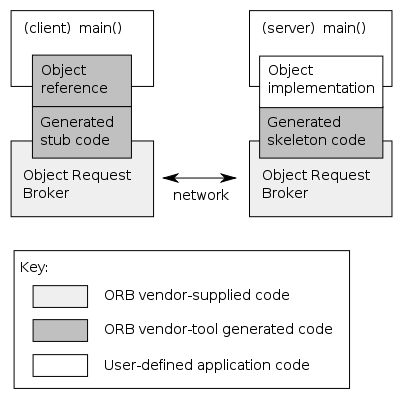
\includegraphics[width=13cm,height=7cm]{401px-Orb.png}
\caption{Model de Client-servidor que necesitem}
\label{fig:401px-Orb.png}
\end{figure} 

Tecnologíes per a executar RPCs (Remote procedure call) n'hi ha moltes
diferents. Les tecnologies que ens obliguen a utilitzar el mateix llenguatge de
programació han quedat descartades de bon principi, ja que un dels objectius
principals és precisament obrir el programa a futures aplicacions que puguem
crear.  És per això que RMI, que ens lliga a java no pot ser utilitzada.  

Una altra alternativa que hem estudiat és CORBA, que és un sistema molt extès
per a tipus d'aplicacions client-servidor en xarxa, i proporciona una capa
intermitja molt còmoda i extensible.  CORBA és un sistema disenyat per a
comunicar diferents llenguatges entre si.  Per aquesta part, ens serveix per als
nostres requeriments, però el protocol de CORBA funciona utilitzant ports TCP
no estàndars, i fa que no poguem garantir la conectivitat si el client o bé el
servidor estàn darrere d'un tallafocs (firewall).

La aplicació Chiron ha de funcionar a través d'una interfície web que estarà
allotjada en un servidor local, i nosaltres controlem la xarxa, però com que
part de la essència de Chiron és el sistema de algorismes genètics genèric, no
volem limitar-nos a la utilització únicament per web.  Per això, s'han seguit
buscant alternatives.

Per asegurar que no tenim bloquejos en la xarxa, hi ha sistemes disenyats per a
treballar només a través de ports coneguts, i normalment oberts en cualsevol
xarxa amb conexió a internet.  Exemples d'aquestes tecnologies son XML-RPC, REST
i SOAP.
% subsubsection Webservice d'Algorismes genètics (end)

\subsubsection{Diseny global} % (fold)
\label{ssub:Diseny global}

Després de diverses iteracions sobre el diseny, la estructura global que ha
quedat del projecte \texttt{Chiron} és la mostrada en la Figura \ref{fig:disenyChiron}.

Chiron es pot integrar en altres programes ja existents de l'empresa, donant
suport amb els algoritmes evolutius.  (XXX: El diagrama s'ha de fer més
específic per a Chiron).

\begin{figure}[h]
	\begin{center}
		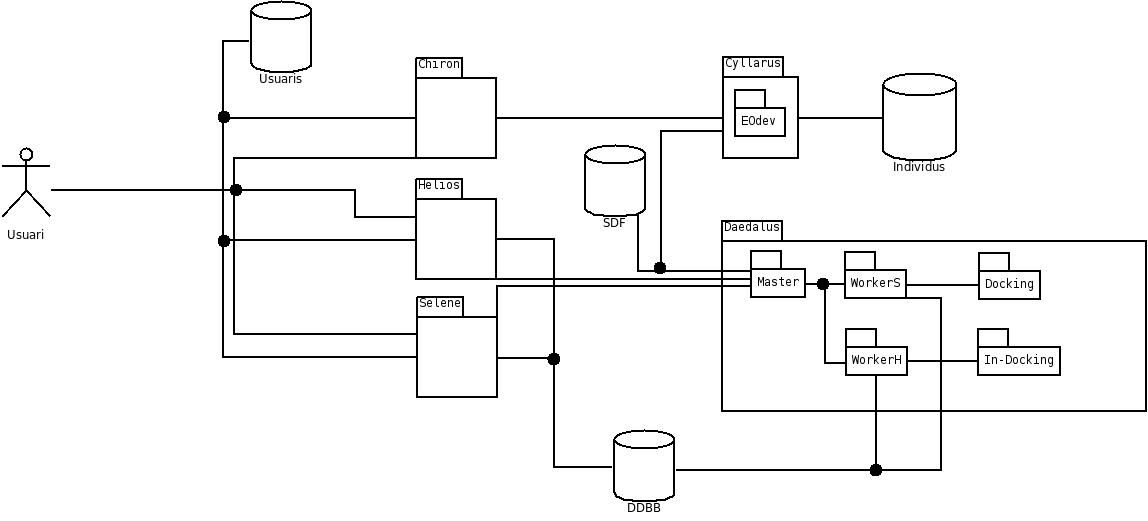
\includegraphics[scale=0.4]{chiron/arquitectura_global_chiron.jpg}
	\end{center}
	\caption{Es}
	\label{fig:disenyChiron}
\end{figure}
% subsubsection Diseny global (end)

% subsection Funcionament General (end)

\subsection{Algoritme Genètic} % (fold)
	\label{sub:Algoritme Genetic}
% subsection Algoritme Genetic (end)

L'algorisme genètic de Chiron, és un algorisme a ``mig implementar'', en el
sentit que  al ser parametritzable en quant a la funció de fitness, li falta una
de les parts principals dels algorismes genètics.  Això no vol dir que no haguem
implementat la funció de fitness, sinó queda externalitzada respecte el nucli de
\texttt{Chiron}.  Tot seguit s'explica la implementació de cadascun dels
parametres i estructures de dades necessàries per a la implementació de Chiron.

\subsubsection{Inicialització} % (fold)
\label{ssub:Inicialitzacio}

En  molts casos reals, ens trobem que tenim una immensa majoria de valors iguals
com a resultat de les evaluacions.  Aquests resultats són per les molècules que
o bé no poden ser sintetitzades, o bé no superen un llindar mínim d'activitat.

Això ens ha suposat un gran problema perquè si evaluem la primera generació i
tots els elements tenen el mateix fitness (0), la següent població que Chiron
suggerirà serà una població tal que haurà sortit de creuar i mutar la primera
població aleatoriament entre ella.  Aquest procediment ens provoca una
convergència prematura que no desitgem, ja que el que passa en realitat és que
encara no hem mostrejat cap molècula que ens doni un mínim d'activitat amb el
que poder ``jugar''.

Problemes d'aquestes característiques només es donen en casos on l'espai de
búsqueda és molt gran comparat amb el número de elements que tenen resultats
diferents de 0.

Per exemple, si volguéssim trobar, en el problema de la suma de bits una
configuració concreta (10101), o bé trobar elements amb unes certes
característiques (que sumin 3), i tots els elements que ho compleixen tenen
fitness 1 i els que no, tenen fitness 0, ens trobariem amb problemes similars.

Aquest problema, l'hem solucionat provocant que Chiron resetegi l'experiment
(recordant les molècules evaluades en la base de dades), i torni a donar una
població d'individuus aleatòria.  Així maximitzem les probabilitats de trobar un
o més pous energètics, que son les àrees del espai de búsqueda (normalment
contígues) on es troben els elements amb fitness superiors al llindar.  En el
moment que trobem molècules amb activitat, l'algorisme segueix el procediment
normal.

% subsubsection Inicialització (end)

\subsubsection{Individu (Cromosoma)}
\label{ssub:individu (cromosoma)}

En aquest algorisme genètic, els indicis són les diferents combinacions de
ramificacions, en cadascuna de les posicions. Com que els canvis entre un al·lel i un
altre són qualitatius, cada posició del cromosoma és un enter, que representa
una terminació diferent en funció de la posició on es troba dins el cromosoma.

Així doncs, tenim un vector de N posicions on N és el número de ramificacions que té
l'esquelet, i cada posició conté un enter, amb limits d'acord amb les
especificacions del usuari al iniciar el projecte. 

Utilitzem enters per a representar cada al·lel perquè és la forma més comoda que
tenim per represetar valors qualitatius o categòrics.  A més, els valors límit
de cada posició s'acoten en cada projecte.  Això és un altre tret que el
diferència de programes més estatics on els límits són coneguts a priori, com
per exemple Pholus (\ref{cha:Pholus}).

Si els possibles valors adoptats en cada punt fóssin coneguts en temps de
desenvolupament del projecte, es podria usar tipus enumerats, per a deixar ben
clar que els valors són qualitatius i que hi ha la mateixa diferència en un
al·lel entre el valor 1 i el 2 que entre el 1 i el 5, ja que simplement són
ramificacions diferents, i no tenen res a veure un amb l'altre.  Això també ens
condiciona els creuaments, com s'explica en la següent secció.

%PUNT

\subsubsection{Selecció} % (fold)
\label{ssub:CSeleccio}
En aquest problema, hem utilitzat un algorisme de sel·lecció per Torneig
determinista ($p=1$), on competeixen dos individuus.  Donat que les poblacions
són relativament petites en la majoria de casos (tenim un espai total de cerca
de gairebé 16000), hem utilitzat un torneig petit, ja que la presió evolutiva
que implica pujar el torneig en un és molt gran, i de seguida ens estanca en
problemes de convergència prematura.

% subsubsection Selecció (end)

\subsubsection{Crossover} % (fold)
\label{ssub:Crossover}

Com a operador de creuament entre 2 individuus d'una generació, s'utilitza el
tall per 1 punt.  La raó d'això és que cadascun dels al·lels té un valor
cualitatiu, i no té cap sentit fer altres creuaments on el mateix gen (mateixa
posició del vector) es creua físicament amb el gen de l'altre cromosoma.

Un creuament que involucrés aritmètica no es pot fer servir en aquest cas ja que
no es poden sumar ``peres i pomes''.

Creuaments que involucrin el canvi de posició en els gens tampoc eren naturals
per aquest problema, ja que s'hauría de comprovar que cap gen es col·loca en una
posició on no pot ser-hi ja que supera els límits estipulats per la
posició final.  A part d'aquest fet totalment subjecte a implementació, i per
tant, solucionable amb una mica més de comprovacions, aquests creuaments no
tenen sentit químic, ja que l'alternativa $i$ de la posició $n$, no té perquè
tenir res a veure, ni cap correlació amb l'alternativa $i$ de la posició $m$ on
$n <> m$.

Pel creuament s'ha provat un creuament per un punt, i el creuament per dos
punts, donant resultats similars en els dos casos.  Donat que els experiments
químics en què s'ha provat (\ref{sec:Resultats}), tenen només tres llocs per a
substituients, un creuament per diversos punts no tenia gaire sentit.

Donats dos individus (els que han estat sel·leccionats en el procés de
sel·lecció per a reproduir-se , amb una provabilitat d'un 0.8 es fa creuament i
els fills són tan sols una partició formada a partir dels 2 pares, amb un punt
de tall aleatori.  Donat que no hi ha cap relació entre els diferents indexos
(estàn ordenats arbitràriament) no ens hem de preocupar de partir el cromosoma
per lloc ``delicat''. 

Així doncs, el que es busca és interpolar les qualitats de dos individuus ben
adaptats, per a crear uns descendents amb propietats similars.  És d'esperar que
si un individu té bon fitness, les ponderacions donades als seus indicadors
siguin bastant encertades.  Llavors, en interpolar una parella de individuus,
suposem que el descendent també tindrà un fitness bo, i això farà que a mesura
que passen les generacions, la població tendeixi a millorar (en mitja).

En els experiments en formules matemàtiques, ha donat millors resultats el tall
en 2 punts, que no pas en 1.

% subsubsection crossover (end)

\subsubsection{Mutacions} % (fold)
\label{ssub:Mutacions}

La única mutació que té sentit en aquest problema és canviar un dels elements
del cromosoma per un altre, sempre dins del rang que tingui en aquesta posició.

Intercanvis de al·lels de diferents posicions no són possibles ja que les
diferents posicions del cromosoma tenen rangs diferents, i fa que molts dels
intercanvis que fariem siguin invàlids.
% subsubsection Mutacions (end)


\subsection{Implementació} % (fold)
	\label{sub:Implementacio}

Tot seguit es detallen algunes particularitats de la implementació de
\texttt{Chiron}, amb les seves tecnologíes, i algun codi exemplificador del que
s'està explicant.

\subsubsection{Algorisme genètic} % (fold)
\label{ssub:algorisme genetic}

En aquest projecte s'han utilitzat les llibreries eodev, igual que en el
projecte \texttt{Pholus}, ja que ens proporcionen les qualitats suficients per a
poder treballar per sobre d'elles sense haber de fer gaires modificacions sobre
el seu codi base.

Eodev proporciona una estructura genèrica per a algorismes genètics, on, si no
volem massa complicacions, amb un cromosoma de coma flotants, modificant només
la funció de fitness, podem corre ja el nostre algorisme genètic.  Això no ens
serveix per a \texttt{Chiron}, ja que necessitem modificar el cromosoma, les
mutacions i creuaments per al que volem fer nosaltres.

Hem de crear doncs, una classe per a cada element del algorisme genètic.

%PUNT posar totes les classes

% subsubsection algorisme genètic (end)

\subsubsection{Arxius de configuració} % (fold)
\label{ssub:Arxius de configuracio}

Eodev disposa d'una manera per llançar execucions amb un arxiu de configuració
determinat.  El format no respon a cap estàndard (ni .ini, ni .conf\ldots).
Aquest format és el que fem servir per a llançar procéssos \texttt{Chiron}, amb
els parametres adecuats, i per altra banda, entre generació i generació, omplim
els fitness en l'arxiu aquest.  És una manera de colar-se en el procediment de
Chiron, i permetent-nos modificar el fitness d'un element en una generació
determinada.

Per a generar aquest arxiu de configuració hem agafat un dels de demostració que
vénen amb les fonts de Eodev, i hem creat un template o plantilla, utilitzant
Template Toolkit (TT\footnote{\url{http://template-toolkit.org/}}).
%XXX http://oreilly.com/catalog/9780596004767/

Template Toolkit és una llibreria molt extesa per a la generació de textos
parametritzats.  En un principi es va crear per a reproduir textos massivament,
on només canvia una petita part del text (per exemple, circulars), o bé arxius
que han de complir una certa extructura (webs corporatives).

Nostres hem usat la implementació en Perl, que a part de ser la primera que va
sortir (i potser la més sòlida), és el llenguatge en el que hem desenvolupat
tota la part que no forma part del nucli de la aplicació.  Segueix un exemple de
la utilització de Template Toolkit en un cas senzill, i la manera en que ens
facilita la separació de la presentació de la lògica.  És per això que Template
Toolkit també s'utilitza en molts frameworks web perl\footnote{Catalyst.
http://www.catalystframework.org/}.

%codi Template Toolkit
\lstset{language=perl, tabsize=2}
\lstset{commentstyle=\textit}
\lstinputlisting[frame=trbl]{tt.pl}

Encara que en aquest exemple, no sembla més que una versió ``més elegant'' de
sprintf, Template Toolkit pot afegir lògica en les seves plantilles, processant
o no processant arxius en subdirectoris, en funció de valors de variables en el
programa perl que crida les funcions TT.

% subsubsection Arxius de configuració (end)

\subsubsection{DBIx::Class} % (fold)
\label{ssub:DBIx Class}

Tant l'arxiu de configuració de cada projecte, com la informació dels individuus
que han aparescut en generacions passades del projecte, i com el propietari de
cada projecte es mantenen en una base de dades MySql.

La decisió de MySql o bé PosgreSql, no ha estat una decisió on hi hagi hagut un
clar guanyador.  Pel volum de dades que hem de tenir, tampoc creiem que això
sigui una decisió critica per al èxit del projecte, però per si de cas, hem
decidit utilitzar un sistema de ORM \footnote{Object Relational Mapper} .

Els ORMs són llibreries que mapegen taules SQL a objectes del llenguatge, podent
així fer més directe el tractament amb bases de dades desde llenguatges de
programació, fent que no s'hagi de fer un canvi de paradigma tant gran al
canviar de OOP pura a SELECT * FROM \ldots  .

Sabem doncs, que per al projecte, en l'estat actual no és necessari plantejar-se
quina és la millor base de dades a escollir, si hem fet una bona el·lecció pel
que fa a les eines i llibreries, ja que utilitzant DBIx::Class, canviar de SGBD no
suposa cap modificació en el codi, fent-ho del tot transparent.

% subsubsection DBIx\dots Class (end)

\subsubsection{Webservices i Soap} % (fold)
\label{ssub:WS i Soap}

Com ja s'ha explicat anteriorment (\ref{sec:Procediment informatic} ), per a la
comunicació segons el paradigma client-servidor, s'ha utilitzat la tecnologia
SOAP\footnote{Simple Object Access Protocol}.

Els seus rivals més igualats, per als nostres requeriments, han estat XML-RPC i
REST, però hem decidit utilitzar SOAP, entre d'altres coses, perquè és l'únic
que té suport a nivell corporatiu, i no com REST, que son estàndards
desenvolupats majoritàriament en entorns de comunitats Opensource.  Al
utilitzarlo nosaltres en un entorn corporatiu, hem pensat que SOAP seria més
adequat pel possible suport que tindría i la interpolabilitat amb altres
aplicacions que es poden utilitzar en el futur.
%PUNT . POSAR L'ESTANDARD SOAP, I WSDLs i XMLs d'exemple?

% subsubsection Webservices i Soap(end)
% subsection Implementació (end)
% section Procediment informàtic (end)

\section{Resultats} % (fold)
	\label{sec:Resultats}

	En les proves que hem realitzat, \texttt{Chiron} ha donat bons resultats,
	però necessitem fer algunes validacions per a assegurar que ha valgut la
	pena aquest esforç, i també tenir dades objectives sobre la seva utilitat.
	A nivell comercial, també es vol tenir alguna validació estadística que ens
	doni seguretat per a ``vendre'' Chiron.

	Per a realitzar les proves inicials, s'han utilitzat funcions típiques de
	testeig d'algorismes genètics, com la suma de bits (es tracta de maximitzar
	el número de bits a 1 en un vector), o alguna funció trampa, on el màxim de
	la funció no està en cap extrem del espai de búsqueda.

	Les proves sobre un escenari real en el que operarà Chiron, s'han fet sobre
	tres projectes dels quals s'ha realitzat la prova experimental de totes les
	combinacions de substituients possibles (s'han trobat en (XXX Ppaper) )

	En aquests tres problemes, els autors dels experiments van sintetitzar totes
	les possibles molècules, obtenint un resultat de activitat en cadascuna
	d'elles.  És possible que algunes d'elles fóssin impossibles de sintetitzar,
	i que els hi haguéssin posat un fitness molt baix.  Això ja ens va bé per
	als nostres propòsits, ja que és el mateix resultat que els hi donaríem
	nosaltres.

	Per a testejar Chiron, hem usat un programa de test, que analitza totes les
	dades experimentals, tenint així una resposta per a cada possible individuu
	que pugui proposar Chiron.

	Aquest programa de prova, ha estat desenvolupat en Perl, atacant directament
	la llibrería també programada en perl, no pas usant la interfície SOAP, ja
	que podent fer les proves en local, és molt més ràpid en executar-se.

	S'han fet 25 executions executions de Chiron per a cada projecte, i hem
	esperat a què convergeixin cadascun dels 3 projectes.  Com que tenim a la
	nostra disposició totes les dades del espai de búsqueda, hem fet càlculs
	respecte quantes avaluacions s'han fet fins a trobar el millor element que
	hem arribat a trobar.  També ens fa falta saber quin és el fitness d'aquest
	element, i quin és el fitness de la millor combinació de substituients que
	hi ha en tot l'espai de búsqueda. 

	%TAULA de resultats.

% theme=Berlin;caption_top=1;caption=Exemple tanimotos
% BBDD & Fitness & Elements avaluats & relació

%png('file.png')
%hist(x)
%dev.off()

	A continuació es mostren les validacions que s'han fet a chiron.  

	%XXX XAVI

	\begin{figure}[tbp]
		\begin{center}
			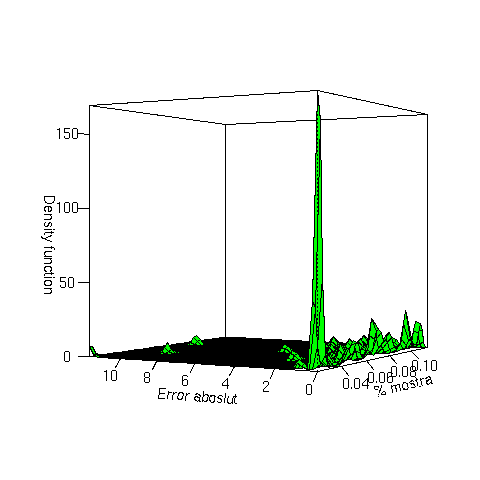
\includegraphics[scale=0.75]{chiron/rgrau1.png}
		\end{center}
		\caption{Resultat Chiron 1}
		\label{fig:resChir1}
	\end{figure}

	\begin{figure}[tbp]
		\begin{center}
			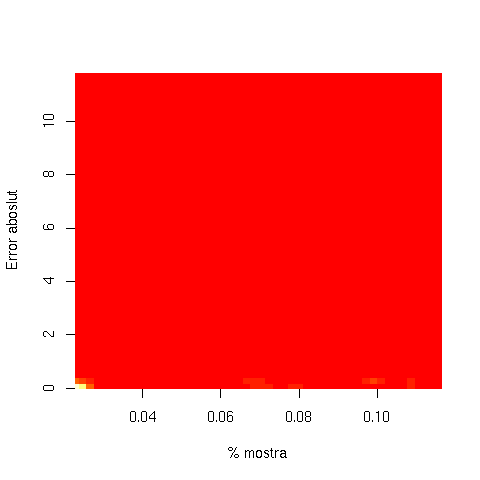
\includegraphics[scale=0.75]{chiron/rgrau2.png}
		\end{center}
		\caption{Resultat Chiron 2}
		\label{fig:resChir2}
	\end{figure}

	\begin{figure}[tbp]
		\begin{center}
			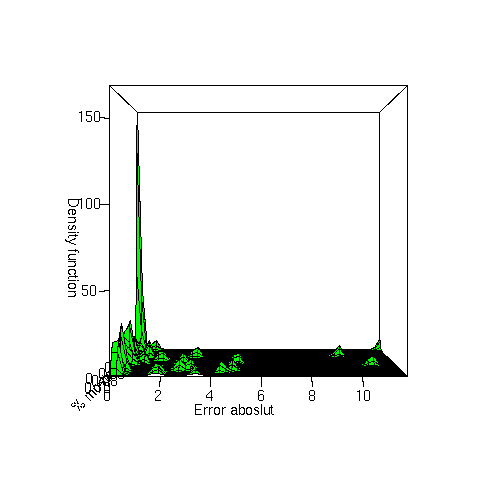
\includegraphics[scale=0.75]{chiron/rgrau3.png}
		\end{center}
		\caption{Resultat Chiron 3}
		\label{fig:resChir3}
	\end{figure}
	\begin{figure}[tbp]
		\begin{center}
			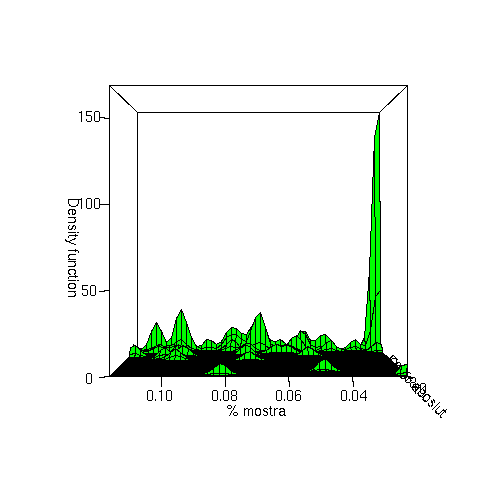
\includegraphics[scale=0.75]{chiron/rgrau4.png}
		\end{center}
		\caption{Resultat Chiron 3}
		\label{fig:resChir4}
	\end{figure}

	Aquestes gràfiques mostren, de diferents maneres, el nombre de elements
	avaluats, i l'error absolut que s'ha obtingut en cadascun dels experiments.

	La intenció inicial era utilitzar l'error relatiu, però en aquests
	experiments, els pitjors fitness tenen un valor de infinit.  Com que els
	tres experiments sobre els que hem fet les proves són molt similars en quant
	al millor fitness possible (0, 0.1 i 0.01 XXX), hem pogut disenyar un
	sistema de tests unificant els resultats dels tres experiments, i així tenir
	una idea més general del rendiment de \texttt{Chiron}.

	Com ja s'ha dit prèviament, s'han  realitzat 25 execucions de cadascun dels
	tres experiments, guardant per a cadascun el número d'individuus que s'han
	avaluat, el número total d'individuus del espai de cerca, el millor fitness
	de tot l'espai de cerca, i el millor fitness al que hem arribat.

	D'aquesta manera, hem pogut fer un estudi estadístic sobre el funcionament i
	rendiment de Chiron.

	L'estudi, estadístic, l'hem realitzat utilitzant el software estadístic
	R(\url{http://www.r-project.org/}), i ens permet dir coses com per exemple, que \textbf{avaluant un XXX
	\% de l'espai de búsqueda, ens quedem a XXX del millor en un XXX dels casos}


\subsection{Conclusions i treball futur} % (fold)
	\label{sub:CConclusions i treball futur}

	Els resultat de \texttt{Chiron} és satisfactori, però com a projecte futur
	d'ampliació, està implementar tècniques de algorismes genètics interactius.

	Donat que la avaluació és supervisada per l'usuari, podriem implementar
	tècniques per a classificar els individuus de cadascuna de les generacions,
	per a només donar al usuari una part de la població a avaluar, en funció de
	la semblança entre els individuus.  Es podria utilitzar alguna tècnica de
	clustering, o eines més particulars d'algorismes genètics interactius, com
	per exemple (XXX paper company natxo).
	% subsection treball futur (end)
% section Resultats (end)

%\end{document}
%# vim: set tabstop=4 shiftwidth=4 tw=80 foldmethod=marker ignorecase : ##
